%
% File acl2015.tex
%
% Contact: car@ir.hit.edu.cn, gdzhou@suda.edu.cn
%%
%% Based on the style files for ACL-2014, which were, in turn,
%% Based on the style files for ACL-2013, which were, in turn,
%% Based on the style files for ACL-2012, which were, in turn,
%% based on the style files for ACL-2011, which were, in turn, 
%% based on the style files for ACL-2010, which were, in turn, 
%% based on the style files for ACL-IJCNLP-2009, which were, in turn,
%% based on the style files for EACL-2009 and IJCNLP-2008...

%% Based on the style files for EACL 2006 by 
%%e.agirre@ehu.es or Sergi.Balari@uab.es
%% and that of ACL 08 by Joakim Nivre and Noah Smith

\documentclass[11pt]{article}
\usepackage[english]{babel}
\usepackage{acl2015}
\usepackage{times}
\usepackage{url}
\usepackage{latexsym}
\usepackage{graphicx}
\usepackage{subcaption}
\usepackage[english]{babel}
\usepackage{fancyhdr}

\pagestyle{fancy}
\fancyhf{}
\fancyhead[RE,LO]{}
\fancyhead[RE,LO]{}
\fancyfoot[CE,CO]{CS230 Stanford University Project Milestone}
\fancyfoot[LE,RO]{\thepage}
\renewcommand{\headrulewidth}{0pt} 

\setlength\titlebox{3cm}

% You can expand the titlebox if you need extra space
% to show all the authors. Please do not make the titlebox
% smaller than 5cm (the original size); we will check this
% in the camera-ready version and ask you to change it back.


\title{Learning to Play Minichess Without Human Knowledge}

\author{
  { Karthik selvakumar Bhuvaneswaran} \\
  {\tt karthik0@stanford.edu}
}

\date{May 19th 2018}

\usepackage{listings}
\usepackage{color}

\definecolor{dkgreen}{rgb}{0,0.6,0}
\definecolor{gray}{rgb}{0.5,0.5,0.5}
\definecolor{mauve}{rgb}{0.58,0,0.82}
\lstset{frame=tb,
  language=Python,
  aboveskip=3mm,
  belowskip=3mm,
  showstringspaces=false,
  columns=flexible,
  basicstyle={\small\ttfamily},
  numbers=none,
  numberstyle=\tiny\color{gray},
  keywordstyle=\color{blue},
  commentstyle=\color{dkgreen},
  stringstyle=\color{mauve},
  breaklines=true,
  breakatwhitespace=true,
  tabsize=3
}

\begin{document}
\maketitle
\begin{abstract}

Implementing a self play based algorithm using neural networks has become popular after the tremendous success of Alpha Zero by Deep Mind in the game of go. Replicating the results for a game with smaller search space like TicTacToe, Connect4 etc has already been proven in alpha-zero-general, but for games with larger search space like chess requires scaling.
In this paper we apply scaled up version of alpha-zero-general for the game of Minichess and evaluate our learning algorithm with random and greedy baselines. 

\end{abstract}


\section{Introduction}

It was estimated that games like Go, which have a large branching factor, and where it is very difficult to determine the likely winner from a non-terminal board position, would not be solved for several decades. However, AlphaGo (Silver et al. 2016), which uses recent deep reinforcement learning and Monte Carlo Tree Search methods, managed to defeat the top human player, through extensive use of domain knowledge and training on the games played by top human players. Many of the existing approaches for designing systems to play games relied on the availability of expert domain knowledge to train the model on and evaluate non-terminal states. Recently, however, AlphaGo Zero (Silver et al. 2017b) described an approach that used absolutely no expert knowledge and was trained entirely through self-play. This new system, AlphaGo Zero, even outperforms the earlier AlphaGo model. This represents a very exciting result, that computers may be capable of superhuman performances entirely through self-learning, and without any guidance from humans. In our work, we extract ideas from the AlphaGo Zero paper and apply them to the game of Minichess. We use board sizes of 5x5 with different board layouts, for which learning through self-play took 5 to 7 days in a single CPU/GPU (with several random crashes), but can be trained within a day with a distributed setup of multiple CPU/GPU. For evaluation, we compare our trained agents to random and greedy baselines.

\section{Related Work}

Self-play for learning optimal playing strategies in games has been a widely studied area. For example, 9x9 Go has been studied in (Gelly and Silver 2008). Chess, though widely played using alpha-beta search strategies, has also seen some work through self-play methods in (Heinz 2001). For the 5x5 version of chess, a perfect strategy for player 2 is known to exist 1. (Silver et al. 2016) and (Silver et al. 2017b) have trained a novel neural network agent to achieve state of the art results in the game of Go. This approach has also been extended to a general game-playing strategy in (Silver et al. 2017a), achieving state of the art in the games of Chess and Shogi. 

\subsection{Deep Mind and Alpha Zero General}
DeepMind published a ​paper​ of Alpha Zero on arXiv that extends AlphaGo Zero methods to Chess and Shogi. However, the code is not open source and will not be released by DeepMind. Moreover, they use about 5000 TPUs to generate games in parallel. This makes it very difficult to replicate the results and extend the work to other games. ​Alpha Zero General​ is open source single-thread single-GPU version that works for any game and any framework (currently PyTorch, TensorFlow and Keras). It works quite well on small games such as 6x6 Othello after ​2-3 days of training on a single GPU​. We will be extending Alpha Zero General project by analyzing the components that can be parallelized and training a Neural Network for the game of Minichess. 

\subsection{Scaling Up the implementation}
  We used tensorflow framework for the implementation. These are key components that can be parallelized: 
\begin{itemize}
\item[1] Training models using distributed batches 
\item[2] Distributed self-play with synchronization  
\item[3] Asynchronous version of MCTS as mentioned in DeepMind paper 
\end{itemize}

 This parallelized implementation will be used to self train Minichess and will be tested based on the results of the game between greedy and random players.

\section{Methods}

We provide a high-level overview of the algorithm we employ, which is based on the AlphaGo Zero (Silver et al. 2017b) paper. The algorithm is based on pure self-play and does not use any human knowledge except knowing the rules of the game. At the core, we use a neural network that evaluates the value of a given board state and estimates the optimal policy. The self-play is guided by a Monte-Carlo Tree Search (MCTS) that acts as a policy improvement operator. The outcomes of each game of self-play are then used as rewards, which are used to train the neural network along with the improved policy. Hence, the training is performed in an iterative fashion- the current neural network is used to execute self-play games, the outcomes of which are then used to retrain the neural network. The following sections describe the different components of our system in more detail. 

\subsection{Distributed Architecture}

We will provide a high level overview of the distributed setup we used to train Minichess. Our experiments were ran on AWS EC2 instances, but architecture can be used even for other cloud services. 

\begin{figure}[h!]
  \centering
  \begin{subfigure}[b]{1\linewidth}
    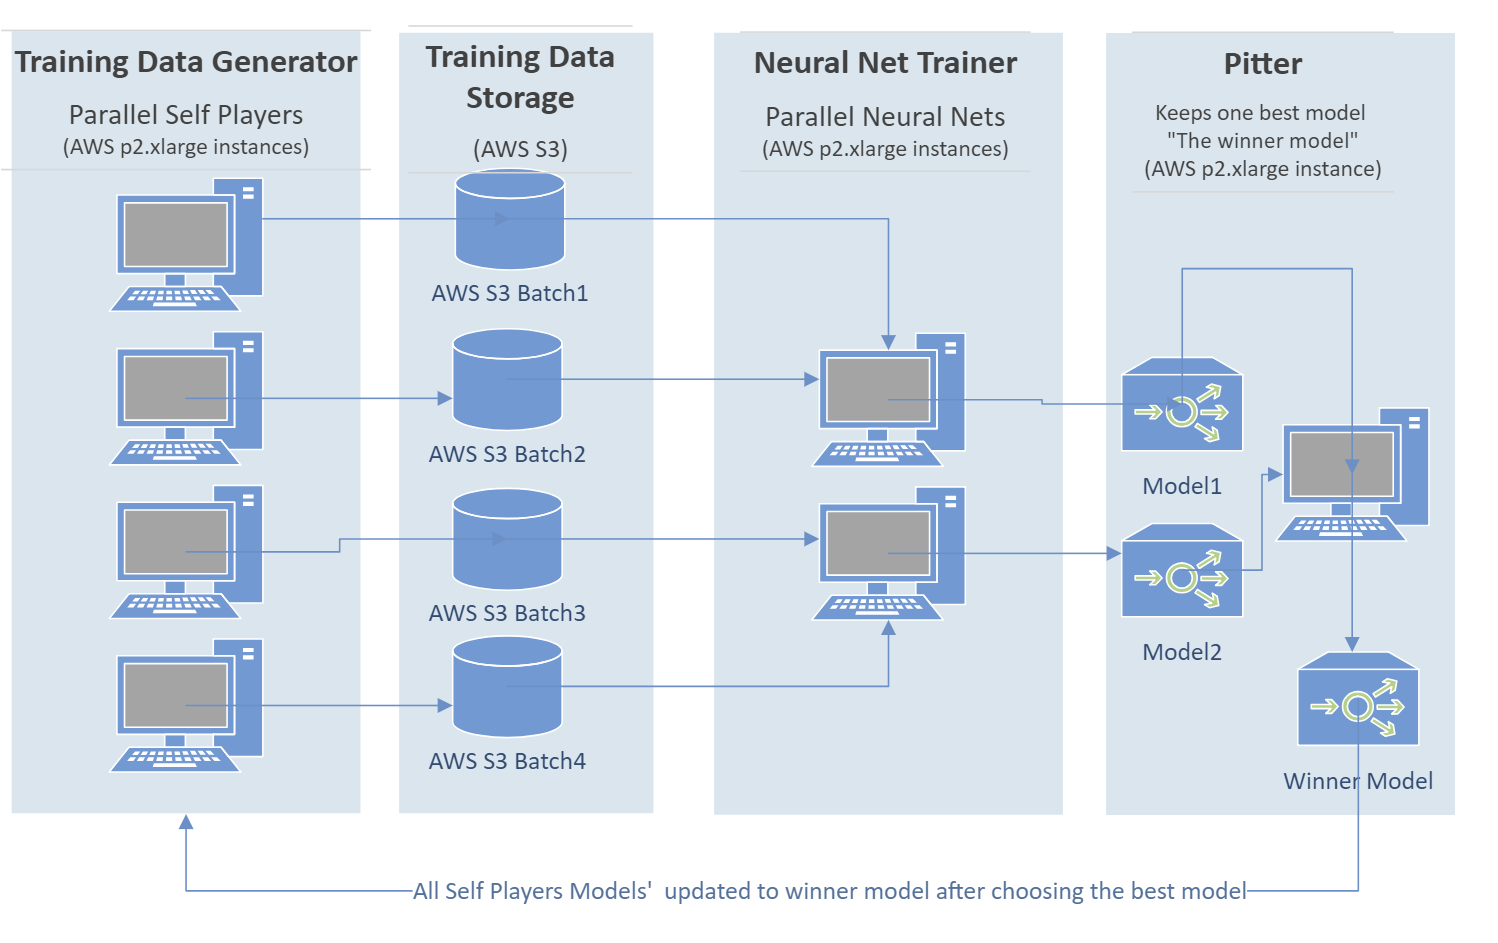
\includegraphics[width=\linewidth]{distributed_arch.png}
  \end{subfigure}
  \caption{Distributed Architecture in AWS}  
  \label{fig:distributed_arch}
\end{figure}


\section{Experiments}

The above sections describe a general approach to game-playing. In our experiments, we specifically tackled the problem of learning to play the game of Othello. Othello is traditionally played on an 8x8 sized board. The size of the state space is exponential in the size of the board. Experimentally, we found that converging to an optimal policy on the 8x8 board with limited computing resources would take a very long time. In order to show the effectiveness of our approach, we also ran experiments on a 6x6 version of Othello 3. The 8x8 version was trained with 50 simulations of the MCTS per step, while the 6x6 version was trained with 25. Both were trained on training examples of 100 episodes per training iteration. The 6x6 version completed 78 iterations of training, while the 8x8 version completed 30 iterations of training. Both were trained for over 72 hours on a Google Compute Engine instance with a GPU.


\begin{table}[h]
\begin{center}
\begin{tabular}{c c c c}
\hline \bf Baseline & \bf Gardner  & \bf Jacobs–Meirovitz & \bf Mallet \\ \hline
Random & 20/20 & 20/20 & 20/20 \\
Greedy & - & - &  \\
Minimax & - & - & \\
Human & - & - & \\

\hline
\end{tabular}
\end{center}
\caption{\label{font-table} Performance on 5X5 chess layouts }
\end{table}

\section{Length of Submission}
\label{sec:length}

Long papers may consist of up to 8 pages of content, plus two extra
pages for references. Short papers may consist of up to 4 pages of
content, plus two extra pages for references.  Papers that do not
conform to the specified length and formatting requirements may be
rejected without review.


% include your own bib file like this:
%\bibliographystyle{acl}
%\bibliography{acl2015}

\begin{figure}[h!]
  \centering
  \begin{subfigure}[b]{0.7\linewidth}
    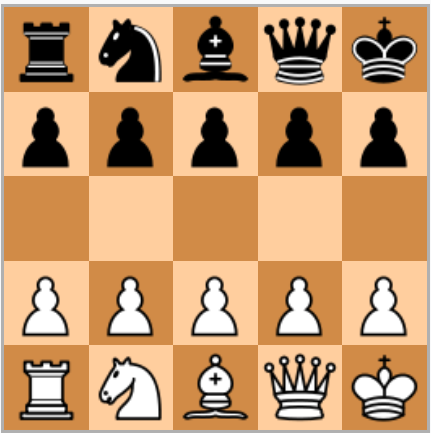
\includegraphics[width=\linewidth]{gardner.png}
    \caption{Gardner Chess layout 5X5}
  \end{subfigure}
  \begin{subfigure}[b]{0.7\linewidth}
    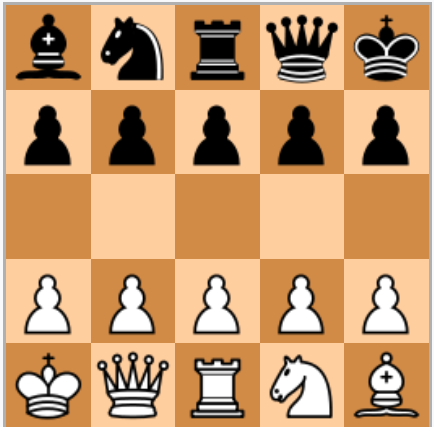
\includegraphics[width=\linewidth]{jacobs.png}
    \caption{Jacobs–Meirovitz Chess layout 5X5}
  \end{subfigure}
  \begin{subfigure}[b]{0.7\linewidth}
    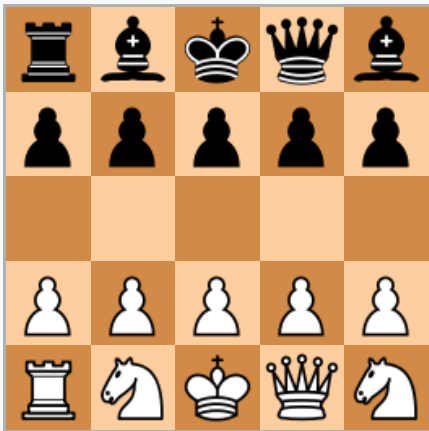
\includegraphics[width=\linewidth]{wallet.png}
    \caption{Mallet Chess layout 5X5}
  \end{subfigure}
  \caption{Different Chess Layouts for 5X5 board}  
  \label{fig:coffee}
\end{figure}

\begin{thebibliography}{}

\bibitem[\protect\citename{Aho and Ullman}1972]{Aho:72}
Alfred~V. Aho and Jeffrey~D. Ullman.
\newblock 1972.
\newblock {\em The Theory of Parsing, Translation and Compiling}, volume~1.
\newblock Prentice-{Hall}, Englewood Cliffs, NJ.

\bibitem[\protect\citename{{American Psychological Association}}1983]{APA:83}
{American Psychological Association}.
\newblock 1983.
\newblock {\em Publications Manual}.
\newblock American Psychological Association, Washington, DC.

\bibitem[\protect\citename{{Association for Computing Machinery}}1983]{ACM:83}
{Association for Computing Machinery}.
\newblock 1983.
\newblock {\em Computing Reviews}, 24(11):503--512.

\bibitem[\protect\citename{Chandra \bgroup et al.\egroup }1981]{Chandra:81}
Ashok~K. Chandra, Dexter~C. Kozen, and Larry~J. Stockmeyer.
\newblock 1981.
\newblock Alternation.
\newblock {\em Journal of the Association for Computing Machinery},
  28(1):114--133.

\bibitem[\protect\citename{Gusfield}1997]{Gusfield:97}
Dan Gusfield.
\newblock 1997.
\newblock {\em Algorithms on Strings, Trees and Sequences}.
\newblock Cambridge University Press, Cambridge, UK.

\end{thebibliography}

\end{document}